\documentclass[11pt,a4paper]{article}

\usepackage[utf8]{inputenc}
\usepackage{amsmath}
\usepackage{amsfonts}
\usepackage{amssymb}
\usepackage{apacite}
\usepackage{graphicx}
\usepackage{tikz}
\usepackage{fullpage}
\usepackage{listings}
\usepackage{perpage}
\MakePerPage{footnote}
\usepackage[font=scriptsize,labelfont=bf]{caption}
\usepackage[left=2cm,right=2cm,top=2cm,bottom=2cm]{geometry}

\begin{document}
\title{A Technical Note on calculating charge state abundances in neutron star mergers}
\author{Pranav Nalamwar\footnote{nalamwar@frib.msu.edu}\\FRIB: \url{https://frib.msu.edu}\\Facility for Rare Isotope Beams\\Michigan State University\\Version: 0.02} 
\date{\today}
\maketitle

\noindent{{\Large  \underline{\textbf{Table of Contents}}}}

%make sure to look up table of content syntax


\pagebreak
\noindent{{\Large  \underline{\textbf{Big Picture Intro}}}}
\par 
Supernovae, or the explosions marking the deaths of heavy stars, formed the heavier elements through the rapid neutron capture process, or r-process(see Fig.1 for formed elements). Nuclei capture neutrons in a neutron-rich environment, creating a radioactive isotope that later decays into stable ones. However, a new class of astronomical event seems to be the source of the remaining r-process elements: neutron star mergers. These neutron star mergers(NSMs) are often the most neutron-rich events in the universe, so they are necessary for the formation of the rather heavy elements, most notably the lanthanides and actinides. Understanding all the details to this event will uncover why there is a large abundance of elements like gold and uranium. There have been two confirmed NSMs, most notably GW170817 in 2017. This merger also had an associated kilonova, the optical transient AT2017gfo. The kilonova light curve, which shows its brightness over time, is a direct result of r-process elements, especially the lanthanides. How bright and in what wavelengths the kilonova is in is determined by the composition and distribution of the lanthanides. By studying its optical spectra(from here on, spectra refers to optical spectra), one can deduce which elements were created in the merger event as these atoms emit light contributing to this observed spectra.\par 

Understanding how the r-process operates in NSMs is necessary to detailing how these heavy elements form. Our goal is to look at which ionization states and isoelectronic states of which elements dominate the merger mixture at late times. Between 1 hour to 2 weeks after the merger, many of the newly formed isotopes don’t have significant variations in their abundance, indicating they contribute both to the optical spectra observed and the overall abundance of the heavy elements. The kilonova light curve for GW170817 is rather detailed but due to the numerous contributing lines present, the ionization states specific to the lanthanides that are important to the late time merger material should be studied. Many NSM and kilonova codes use varying atomic databases for opacity and spectra calculations, so by uncovering which ionization states are important, we can measure their properties in a laboratory to benchmark all the atomic calculations used by these codes. 
\\\\
\noindent{{\Large  \underline{\textbf{Attacking the Problem}}}}
\\\\
To accurately produce the necessary charge state abundances for the elements in consideration, the Saha equation is utilized. The Saha equation relates the abundances of different charge states of one element based on the temperature, electron fraction, ionization potential, and density. Skynet \cite{lippuner2017skynet}, a nuclear reaction network code designed to output isotopic abundances of r-process elements formed from neutron star mergers, is utilized in conjunction with the Saha equation. The derivation is provided below.
\newpage

\maketitle   This sheet uses the Saha equation to find out the charge state abundances based solely on data provided by Skynet.
\\
\\
We start with the constraint on the element abundances of element Z. Essentially, for a given timestep, the sum of all ionization state abundances will equal the elemental abundance provided by Skynet. Technically, Skynet provides data in isotopic abundances, so the sum of the isotopic abundances of any element is the elemental abundance. The element is determined purely by the number of protons:
$$Y_Z (t) = \sum_{I=0}^{Z} Y_{Z,I}(t)$$
where $Y_Z (t)$ is the total abundance of element Z and $Y_{Z,I}$ is the abundance of Z in ionization state I.
\\
\\
$$Y_{e,bound} = \sum_{Z=0}^{Z_{max}} \sum_{I=0}^{Z} (Z - I) Y_{Z,I}(t) = (1-f) Y_{e,tot}(t) $$
Note: $Z_{max}$ is for summing over all possible elements while the second sum is summing over all possible ionization states of Z. 
\\The value of $f$ is introduced such that $Y_{e,free} = f Y_{e,tot}$, where $Y_{e,free}$ is the electron free fraction and $Y_{e,tot}$ is the total electron fraction in the mixture, both of which are fractions between 0 and 1. However, since $f$ is an expensive calculation, just note $f$ as a fraction between 0 and 1. This value will be calculated later in the Saha python class. 
\\\\Let's now take the Saha equation, which is converted to abundances rather than densities: $$\frac{Y_{Z,I+1}}{Y_{Z,I}}  = \frac{2}{\rho N_A * Y_{e,tot}*f}  \left(\frac{G_{Z,I+1}}{G_{Z,I}}\right) \left(\frac{m_e k_b T}{2\pi\hbar^2}\right)^\frac{3}{2} \scalebox{1.3} e^{\left(\frac{\displaystyle -\chi_i}{\displaystyle k_b T}\right)} $$ \

Note: $\rho = $ density of outgoing ejecta in $g/cm^3$, $N_A = $ Avogadro's Number = $6.02214076*10^{23} \hspace{.1 cm} mol^{-1}$, $m_e = $ mass of an electron, $9.109 * 10^{-28} \hspace{.1 cm} g $, $k_b = $ Boltzman Constant = $1.38064852 * 10^{-16} \hspace{.1 cm} erg/K$, $T = $ temperature in $GK$, $\hbar = $ Reduced Planck's Constant = $1.0545 * 10^{-27} \hspace{.1cm} erg \cdot s$, and $\chi_i = $ Ionization Potential in $eV$.\\
 

The function $G$ is the partition function, but since most of these states are unknown, we cannot focus on it. Instead, we assume the partition function ratio is approximately 1. We will condense the entire right side of the equation into a function $g_i (p,Y_{e,tot},T) $.
\\\\
This next section will purely be calculations and equations: $$ Y_{Z,I+1} = Y_{Z,I} * g_I \Longrightarrow  Y_{Z,1} = Y_{Z,0}*g_0 $$   $$ Y_{Z,2} = Y_{Z,1}*g_1 = Y_{Z,0}*g_1 * g_0 $$
such that 

\begin{align} 
Y_{Z,I} = Y_{Z,0} \prod_{m=0}^{I - 1} g_m 
\end{align}

Put in constraint on $Y_Z$ : $$ Y_Z = \sum_{I=0}^{Z} Y_{Z,0} \left(\prod_{m=0}^{I - 1} g_m\right) $$\\
\begin{align} 
\Longrightarrow Y_{Z,0} = \frac{Y_Z}{\quad \displaystyle \sum_{I=0}^{Z} \medspace \prod_{m=0}^{I - 1} g_m}
\end{align}

Note that the right hand side of the equation can be calculated purely from Skynet output and data about ionization potentials, which means you can use equation (1) to get all the $Y_{Z,I}$ for a single Z. 
\\
In total, you well have a function like this: $$func(T,\thinspace p,\thinspace Y_{e,free},\thinspace [\chi_i],\thinspace Y_Z)$$
Now, while these equations are correct, they do result in overflow and underflow issues when graphing the abundances towards the very beginning of the abundance calculations. Therefore, instead of altering the ionization state each time $g_m$ is calculated, focus on just one ionization state. 
\\\\
Rewrite the expression  $\thinspace \displaystyle \prod_{m=0}^{I - 1} g_m$ as $h_I$, which is a function of $T,\thinspace p,\thinspace Y_{e,free}$ \\\\
Then, $Y_{Z,I} = h_I  Y_{Z,0}$. Say another ionization state j is chosen, thus $Y_{Z,J} = h_J  Y_{Z,0}$ \\Therefore, the relation $\frac{Y_{Z,I}}{Y_{Z,J}} = \frac{h_I}{h_J} $ $\Longrightarrow
Y_{Z,I} = Y_{Z,J}\thinspace \frac{h_I}{h_J}$ \\\\
We can finally rewrite the elemental abundance $Y_Z$ as $Y_Z =\thinspace \displaystyle \sum_{I=0}^{Z} Y_{Z,I} = Y_{Z,J}\thinspace \displaystyle \sum_{I=0}^{Z} \frac{h_I}{h_J} $.\\ Rewriting this gives 
\begin{align}
Y_{Z,J} = \frac{Y_Z}{\displaystyle \sum_{I=0}^{Z} \frac{h_I}{h_J}}
\end{align} 
Equation (3) follows the same structure as equation (2). In fact, they are identical for J=0. The main difference is that equation (3) utilizes a constant $h_J$, indicating the calculation need not go through every element but only it's own element. This helps solve overflow and underflow issues for early times/high temperatures during the r-process. \\\\
Equation (3) is useful in finding the electron fraction and the charge state abundances for each time step. To do these calculations, only one element was chosen at first:Samarium since the data and the abundance shapes were compared to
 \cite{fontes2017linesmeared}. Two elements were then used, Sm and Eu, in a multiple element mixture calculation. Once this was checked for validity, the abundance function, which requires user input for the number of elements they want, was constructed. \\

\noindent{{\Large  \underline{\textbf{Code Breakdown}}}}
\\\\
The abundance function is the culmination of the single and multiple element codes, The first part of the code uses a function called ionization generator. It requires as input an array of elements by their charge number and outputs a multi-dimensional array of each element's ionization potential based on its ionization state. The basic structure of this output is an array of arrays; the first element of the returned ionization potential array is empty, the second element contains all the potentials for hydrogen, and so on. All data is retrieved from a NIST database, which is then put into a .xlsx file in order to be read by the python program. The ionization generator function is needed to remove any odd or empty values present in the database.

Temperature values are taken directly from Skynet, which are calculated for times up to approximately 31.79 years after the merger or at $10^{-2} K$. Skynet truncates the temperature evolution for late times, we a use a monotonic fit, a linear relationship between temperature and time in log-log space, was used instead. To make this fit, numpy.polyfit was used for late times, thus ensuring the most accurate slope. Currently, this is not a function but rather hard-coded, so this must be adjusted to account for varied skynet parameters. Beyond this, we also created two more functions for the temperature evolution: an evolution model assuming a non-adiabatic photon gas and a model assuming there is the photon gas component as well as a baryon component to the energy. These three models are derived below. \pagebreak









\maketitle   This sheet indicates the equations and logic used to make each type of temperature evolution calculation used in the lanthanide abundance calculations. \\

\textbf{Radiation-Based, Adiabatic Model}: This is the simplest scenario where we take Skynet temperature data and apply a simple power law extrapolation. Here, we assumed that the system is purely radiation-dominated and adiabatic. Since Skynet has a cutoff temperature for late times, we first find the last unique temperature, use the previous 300 points to generate a slope in log log space, and calculate temperatures that follow this power law. Mathematically, this is 

\begin{align}
	\dfrac{log(T)}{log(t)} = m 
\end{align}

 where m is the slope, T is the temperature in GK, and t is the time in seconds. Thus
$$ m*log(t) + b = log(T) $$ We can ignore the intercept in the calculations. To find the next temperature, we do
\begin{align}
	m*log(t) + log(T) = log(T')
\end{align}

where T' is the next temperature. \\ \\

\textbf{Photon Gas, Non-Adiabatic}: Here, we attempt to improve upon the first temperature evolution by assuming the composition consists of a photon gas, which implies that we can no longer use an adiabatic expansion here. Thus there is radiation and a photon gas. We will derive a small change in temperature over a small change in time, which is later used in an ODE solver to figure out the temperature evolution. These values are all specific values. This $\frac{dT}{dt}$ is based purely off data from skynet. We first consider the entropy:

\begin{align}
	S = \dfrac{\lambda T^3}{\rho}
\end{align}

where S is the entropy in , T is the temperature in GK at a given timestep, $\rho$ is the density of the material in $\dfrac{kg}{m^3}$, and $\lambda$ is the radiation constant in $\dfrac{J}{m^2 s {GK}^4}$.  We also know that 

\begin{align}
	\dfrac{dS}{dt} = \dfrac{\dot{Q} f}{T}
\end{align}

where $\dot{Q}$ is the heating rate in erg / s / g, and f is an efficiency from 0 to 1. Thus, after taking the derivative of the defined value of S from above, we set the two equations equal: 

$$ \dfrac{dS}{dt} = \dfrac{\dot{Q}}{T} = \dfrac{\lambda}{f} \left(\dfrac{3T^2}{\rho}\dot{T} - \dfrac{T^3}{\rho^2}\dot{\rho} \right),$$ so then
$$ \dfrac{3 \lambda T^2 \dot{T}}{f \rho} - \dfrac{T^3 \lambda}{f \rho^2}\dot{\rho} = \dfrac{\dot{Q}}{T}, $$ move $\dot{\rho}$ term to the right and get 
$$ \dfrac{3 \lambda T^2 \dot{T}}{f \rho} = \dfrac{T^3 \lambda}{f \rho^2}\dot{\rho} + \dfrac{\dot{Q}}{T}, $$ then divide by $\dfrac{3 \lambda T^2}{f \rho} $ to get
$$ \dfrac{\dot{T}}{T} = \dfrac{\dot{Q} f \rho}{3 \lambda T^4} + \dfrac{\dot{\rho}}{3 \rho} $$ Now note that since $ \dot{\rho} = -3t^{-1} \rho $ and $ \rho = \rho_0 (\dfrac{t}{t_0})^{-3} $ where $p_0$ and $t_0$ are the starting densities and times, respectively, we can do 
$$ \dfrac{\dot{T}}{T} = \dfrac{\dot{Q} f \rho_0}{3 \lambda T^4} \left( \dfrac{t}{t_0} \right) ^{-3} - \dfrac{1}{t} $$ Finally, we have our temperature derivative as 

\begin{align}
	\dot{T} = \dfrac{-T}{t} + \dfrac{\dot{Q} f \rho_0}{3 \lambda T^3} 	\left( \dfrac{t}{t_0} \right) ^{-3} 
\end{align}

 An important thing to note here is that the original temperature-time evolution shows up here as the power law term as well as the photon gas term due to the non-adiabatic expansion. As an aside, we define the radiation constant $\lambda$ as $\lambda =  \dfrac{4 \sigma_{sb}}{3}$. As stated before, we take this $\dot{T}$ and use an ODE solver to get the evolution.
\\\\
\textbf{Photon Gas and Baryon Component}: In this model, we now assume there is a radiation component, a photon gas component, as well as baryons that are part of this ejecta mixture. Due to the baryons, it is important to consider the pressures involved from radiation and the baryons themselves. All terms are specific values. Let us first use the first law of thermodynamics to define the derivative of the energy $\dfrac{d \epsilon}{dt}$ as

\begin{align}
	\dfrac{d \epsilon}{dt} = -P \dfrac{dv}{dt} + \dot{q_{nuc}}
\end{align}

where $\epsilon, P, v, \dot{q_{nuc}}$ are the energy of the system, the pressure, the specific volume, and the nuclear heating rate from r-process decays, respectively. Now note that since $ v = \dfrac{1}{\rho} $ in the gas, then $ \dot{v} = \dfrac{-1}{\rho ^2}\dot{\rho} $. Now we also know that the radiation energy  $\epsilon_{\gamma} =\dfrac{a T^4}{\rho}$, where a is the radiation constant from above ($a = \lambda$). Thus the derivative of the energy is 

\begin{align}
	\dfrac{d \epsilon}{dt} = \dfrac{4a T^3}{\rho} \dot{T} - 			\dfrac{a T^4}{\rho^2}\dot{\rho} 
\end{align}

From here, we can also define the energy as part radiation and part baryonic, which would give us 

\begin{align}
	\epsilon = \dfrac{a T^4}{\rho} + \dfrac{3}{2} \dfrac{k_B T}			{m_p} [\sum_{i=0}^{Z} Y_i(t) + Y_e] 
\end{align}

Equation 8's first term is for the radiation energy while the second term is for the baryons. The baryon component consists of a bunch of protons, neutrons, and electrons, which are all part of some elemental abundance or free-floating, which is why we use $Y_i$ and $Y_e$ here. Now $k_B, m_p$ are the boltzmann constant and the baryon mass, respectively. The baryon mass is chosen to be the proton mass for convenience. $Y_i, Y_e$ are the elemental abundance and electron fraction, respectively. The term in the bracket inside equation 8 will be denoted as $\tilde{Y}$ for convenience.\\
We now take the derivative of this energy equation and later set it equal to the equation 6.
$$ \dfrac{d \epsilon}{dt} = \dfrac{4a T^3}{\rho}\dot{T} - \dfrac{a T^4}{\rho^2} \dot{\rho} + \dfrac{3 k_B}{2 m_p} \tilde{Y} \dot{T} + \dfrac{3 k_B}{2 m_p} T \tilde{\dot{Y}} $$ Set both derivatives equal to each other:
$$ \dfrac{P}{\rho^2} \dot{\rho} + \dot{q_{nuc}} = \dfrac{4a T^3}{\rho} \dot{T} -  \dfrac{aT^4}{\rho^2} \dot{\rho} + \dfrac{3 k_B}{2 m_p} \dot{T} \tilde{Y} + \dfrac{3 k_B}{2 m_p} T \dot{\tilde{Y}} $$ From here, we can solve for $\dfrac{dT}{dt}$, which is 

\begin{align}
	\dfrac{dT}{dt} = \dfrac{[ \dfrac{P}{\rho^2} \dot{\rho} + \dot{q_{nuc}} + \dfrac{aT^4}{\rho^2} \dot{\rho} - \dfrac{3 k_B}{2 m_p} T \dot{\tilde{Y}}]} {[\dfrac{4a T^3}{\rho} + \dfrac{3 k_b}{2 m_p} \tilde{Y}]}
\end{align}

Now while this does solve the time derivative of the temperature, we need to consider what the pressure is in terms of Skynet given variables. Thus, we know that the total pressure, $P_{tot}$, is given as $P_{tot} = P_{\gamma} + P_{ideal}$. Since specific volume $v = \rho ^{-1}$, we get the radiation pressure $P_{\gamma} = \dfrac{a T^4}{3}$.\\
Now the ideal gas pressure is a result of all the baryons in the ejecta, which is usually defined as $P_{ideal} = \dfrac{N k_b T}{v}$, where $N$ is the total number of baryons present. The total number of particles comes from the abundance of species $Y_i = \dfrac{n_i}{n_B}$, where $n_i = \dfrac{N_i}{v}$. Note that $n_B$ is the density of baryons present. Thus, we can now calculate the ideal gas pressure: For a given species i,
$$ P_i = Y_i n_B k_b T  = Y_i \rho k_b T$$ Now since $\rho = m_p n_B$, we then can write $P_i = \dfrac{Y_i \rho k_b T}{m_p}$. Putting all the ideal gas components together, we can write 
$$ P_{ideal} = \sum_{i=0}^{Z} P_i + \dfrac{Y_e \rho k_b T}{m_p} $$ The total pressure, written with $\tilde{Y}$, is:

\begin{align}
	P_{tot} = \dfrac{a T^4}{3} + \dfrac{\tilde{Y} \rho k_b T}{m_p}
\end{align} 

Finally, we can write $\dot{T}$ in terms of known values as 

\begin{align}
	\dfrac{dT}{dt} = \dot{T} = \dfrac{ \left(\dfrac{4 a T^4}{3} + \dfrac{\tilde{Y} \rho k_b T}{m_p} \right) \dfrac{\dot{\rho}}{\rho ^2} + \dot{q}_{nuc} - \dfrac{3 k_b}{2 m_p} T \dot{\tilde{Y}} \hspace{.09in})} { \left( \dfrac{4a T^3}{\rho}  + \dfrac{3 k_b}{2 m_p} \tilde{Y} \right)}
\end{align}
With this equation, we know that the temperature evolution is dependent on $Y_i, Y_e, \rho, T, \dot{q_{nuc}, \dot{\rho}}$. Note that $\dot{\tilde{Y}}$ is not the most important calculation here as it is presumed to be rather small. While it can be calculated by simply finding the change in the elemental abundance over time, it is set to 0 for convenience.\\
Now while we did define $\dfrac{dT}{dt}$ above, we can further simplify our expression by removing the density. Since $\rho = \rho_0 \left(\dfrac{t}{t_0}\right)^{-3}$ and $\dot{\rho} = \dfrac{-3 \rho}{t}$, we can rewrite equation (11) as:

\begin{align}
	\dfrac{dT}{dt} =  \dfrac{ -\left( \dfrac{4aT^4}{3 \rho_0} \left (\dfrac{t}{t_0} \right)^3 + \dfrac{k_b T \tilde{Y}}{m_p} \right) \dfrac{3}{t} - \dfrac{3 k_b T \tilde{Y}}{2 m_p} \dfrac{\dot{\tilde{Y}}}{\tilde{Y}} + \dot{q}_{nuc} } {  \left( \dfrac{4 a T^3}{\rho_0} \dfrac{t}{t_0}^3 + \dfrac{3 k_b \tilde{Y}}{2 m_p}\right) }
\end{align}

Equation (12) is the solution since it was assumed that the density, and therefore its derivative, were homologous. Thus, we now have $\dot{T}$ is a function of $(T,t,\tilde{Y}, \dot{\tilde{Y}},\dot{q}_{nuc})$, which are all outputs of Skynet, except for $\dot{\tilde{Y}}$, which is calculated from taking the derivative of the abundances outputted. T is in units of $GK$, t is in $sec$, $\tilde{Y}$ is unitless, $\dot{\tilde{Y}}$ is in units of $\dfrac{1}{sec}$, $\dot{q}_{nuc}$ is initially in $\dfrac{erg}{sec g}$ but later converted to $\dfrac{J}{kg sec}$, and $\rho_0$ is initially in $\dfrac{g}{{cm}^3}$ but is later turned into $\dfrac{kg}{m^3}$ \pagebreak

































\begin{figure}[h!]
  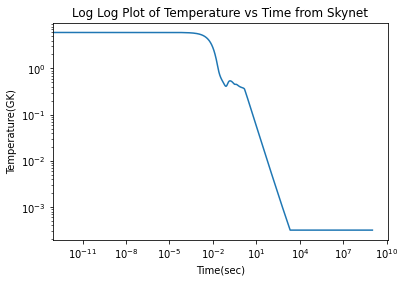
\includegraphics[width=1\textwidth]{skynet_non_linear.png}
  \caption{Plot of temperature vs time with temperature in units of GK. This is data extracted directly from Skynet. For large times, Skynet truncates any temperature calculation, resulting in this flat curve in late times. Temperature ranges from $10^1 \hspace{.03 cm} GK$ to $10^{-4} \hspace{.03 cm} GK$.}
\end{figure}

\begin{figure}[h!]
  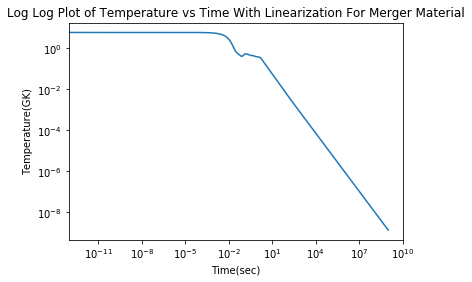
\includegraphics[width=1\textwidth]{temptime.png}
  \caption{Plot of temperature vs time for the merger material after linearizing the plot in loglog space. Note now that the temperature ranges from $10^1 \hspace{.03 cm} GK$ to $10^{-9} \hspace{.03 cm} GK$.}
\end{figure} 

\vspace{1 cm}

The initialization function exists solely to take all the isotopic abundances of a given element and sums it up into the total elemental abundance. For convenience, the output of the function includes the ionization potentials as well as an array of elemental abundances for all the elements in consideration across all times. 

The abundance calculation function uses as input the ionization potentials, the temperature array, the density array, and the total abundances vs time for use in the saha\_mult class. This will return the ionization state abundances for each element across time. Note that each element will contain Z+1 abundance arrays to account for the fully ionized state as well. 

The Saha\_mult class is designed to calculate the free electron fraction of the merger material across time. Skynet outputs the total electron fraction, the temperature array, and the isotopic abundances. Using this, the Saha\_mult class can follow equations (1) - (3) to calculate the ionization state abundances. The most crucial step besides following the equations is finding the $Y_{e,free}$. The main assumption here is that the merger material is charge neutral, indicating the number of protons and electrons must be equal. This allows a Ye contribution to be calculated. Now, using a small and large guess for the $Y_{e,free}$, a bisection method can be used to find the midpoint between the low and high electron fractions. The idea is that this bisection method will eventually calculate a 0 crossing, which will be the actual $Y_{e,free}$. This is done for each timestep, so now the GetAbundancesFixedYef function, which is a form of equation (3), can be used to return all the desired ionization state abundances. Some pseudo code is provided below for context.\\

\noindent{\normalsize{\textbf{Pseudo Code}}}\\
Basic Premise: Set up a way to calculate electron fraction by
considering charge neutrality. Guess some low and high values for a
constant Ye\_free, and plug them into this function to get some range
of possible Ye\_free values. Then, use a bisection method to find the
optimal Ye\_free for when a zero crossing occurs. Using this true
value for Ye\_free, plug into function that returns all ionization
state abundances of the elements of interest. 

\begin{lstlisting}[language=Python]
Yef Contribution Part: 

def GetYefContribution(...): #This will help predict Ye values
	for each element(elements array): 
		Yc = getAbundanceFixedYef(...)
		#Yc = abundance of ionization states assuming constant Ye_f
		for each ion state(element Z+1):
			Ye_free+=Yc * ion_state
			#This finds the number of protons = number electrons
	return Ye_free
			
Bisection Part: #Note all Ye guesses are in log space for convenience

Guess Yef_high = 0 #Max Ye = 1 and log(1) = 0
Guess Yef_low = neg 50 # Any significantly low lnYef will work

if (Yef_high * Yef_low < 0): #Ensure parity are different to do bisection
	for i in range(number of iterations desired):
		mid = avg(high + low)
		check mid*high and mid*low 
		set new low or high depending on any sign changes		
	Ye_free = avg(final_Yef_low + final_Yef_high) #gives final Yef
	
	
	
	
	
Abundance Calculation Part:

for each element in (element array):
	return GetAbundancesFixedYef(... Ye_free)
	#return multiple dimensional array of abundances. Each element
	 contains all ionization state abundances possible, including the
	 free state 
\end{lstlisting}

\vspace{.5 cm}
The plotter function is designed to show 5 unique plots: the relative ionization state abundances of all elements in the mixture vs time and temperature, the relative isoelectronic state abundances(based on number of electrons the atom has), and a graphical check depicting the ratio of the sum of all charge state abundances to the total abundance present. To calculate the relative abundance values, each charge state abundance is divided by the respective elemental abundance. A shift of index by 1 to the right in the ionization state abundance arrays was necessary to form the isoelectronic state abundances.

The final graph is the total abundance of the ionization states vs time. To form this graph, each ionization state abundance is summed together across all the available elements across time. Considering the kilonova peaks around 1 hour to 2 weeks, that became the timescale of these charge state graphs. The graphed formed in the sample code focused solely on the lanthanide abundances.      		
\\\\
\noindent{{\Large  \underline{\textbf{Analysis and Results}}}}
\\\\
The lanthanide graphs reveal many features about how the merger material evolves, especially showing the distribution of elemental and charge state abundances. The elemental abundances in the regime when the kilonova peaks indicates dysprosium as the dominant species. Also, note the fluctuations in each element's abundance. While each species' abundance doesn't change in an order of magnitude, the ranking of lowest to greatest abundance oscillates.

\begin{figure}[h!]
  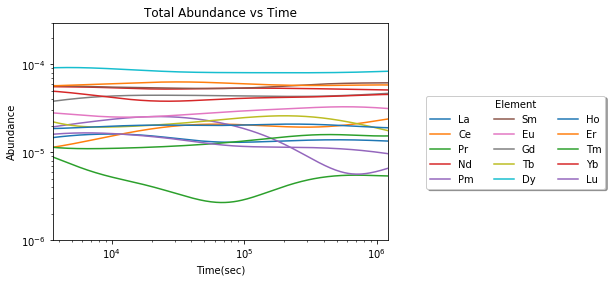
\includegraphics[width=1\textwidth]{elemental.png}
  \caption{Plot of abundances for all lanthanides over time (left) based on output from Skynet. Note that the abundances at early times is noise considering there are values lower than $10-20$. Values become significant around $10^{-1}$ sec}
\end{figure} 

The ionization state abundances can be calculated for any number of elements considered in the mixture, but they all have the same structure. For the test element samarium, it is fully ionized at high temperatures, fully neutral at low temperatures, and changes state in between with multiple peaks representing the point where that specific ionization state is the dominant species for the element.  

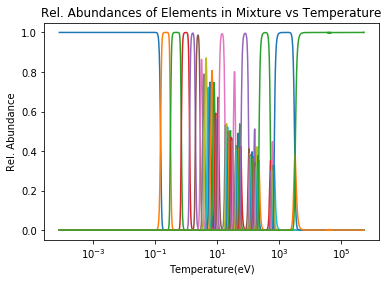
\includegraphics[width=.75\textwidth]{samarium.png}\\
\scriptsize{\textbf{Figure 4:} Relative abundance graph of samarium and 63 unique ionization states vs temperature. Note the changes in the peaks.}\\\\
\normalsize Once all the ionization state abundances were summed up,the plot was limited based on when the kilonova peaks(1 hour to 2 weeks). Much like the individual elements' ionization state plots, the total abundance of ionization state abundances involves numerous peaks indicating the dominant species at a given time. 17 states are considered dominant at late times.

\begin{figure}[h!]
  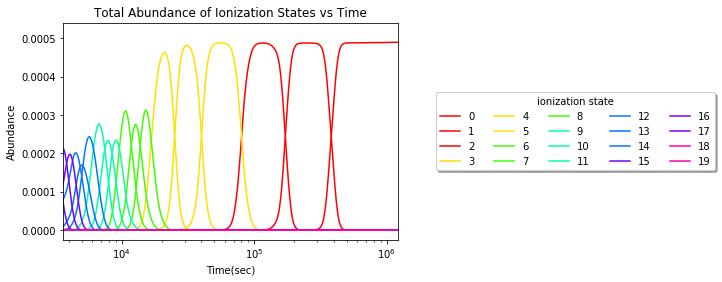
\includegraphics[width=1\textwidth]{total.png}
  \setcounter{figure}{4}
  \caption{Relative abundance graph of all the lanthanides’ ionization state abundances as a function of time in the merger material. The various colors represent the unique ionization states and the first 17 states are dominant at cool temperatures.}
\end{figure}

\newpage

\noindent{{\Large  \underline{\textbf{Conclusion}}}}
\\\\
Based on the analysis of the abundance graphs, many of the lanthanides’ abundances become significant after the r-process occurs. Once this happens, each element undergoes numerous atomic transitions, resulting in certain ionization states to become dominant in the merger material until the neutral state dominates for low temperatures/late times. The total ionization state abundances of the lanthanides indicate that 17 ionization states are important from one hour to two weeks, but only the neutral state and the first two ionization states are significant on the orders of days to weeks. 

\bibliographystyle{apacite}
\bibliography{References}
\end{document}

